\chapter*{Lab 3 - Mesh}

\section{Parte 1 - Blender}
Per questa esercitazione (e per le future) si è scelto di creare una batteria. Le tecniche utilizzate per questa creazione sono state le seguenti:
\begin{itemize}
  \item Extrusion
  \item Spinning
  \item Skinning?
  \item Swinging?
\end{itemize}
Elementi della batteria creati:
  \begin{multicols}{3}
    \begin{itemize}
      \item Grancassa con aste
	  \item Hit-Hat con pedale
	  \item Rack con tutti i sostegni
	  \item Rullante
	  \item Timpano
	  \item Due Tom
	  \item Due Crash
	  \item Ride
	  \item Pedale Grancassa
    \end{itemize}
  \end{multicols}
Il risultato è il seguente. Nella cartella \textit{PART-I/Immagini del processo/} è possibile osservare vari step della creazione.
\begin{figure}[hbt]
    \centering
    \subfloat[Fronte]{{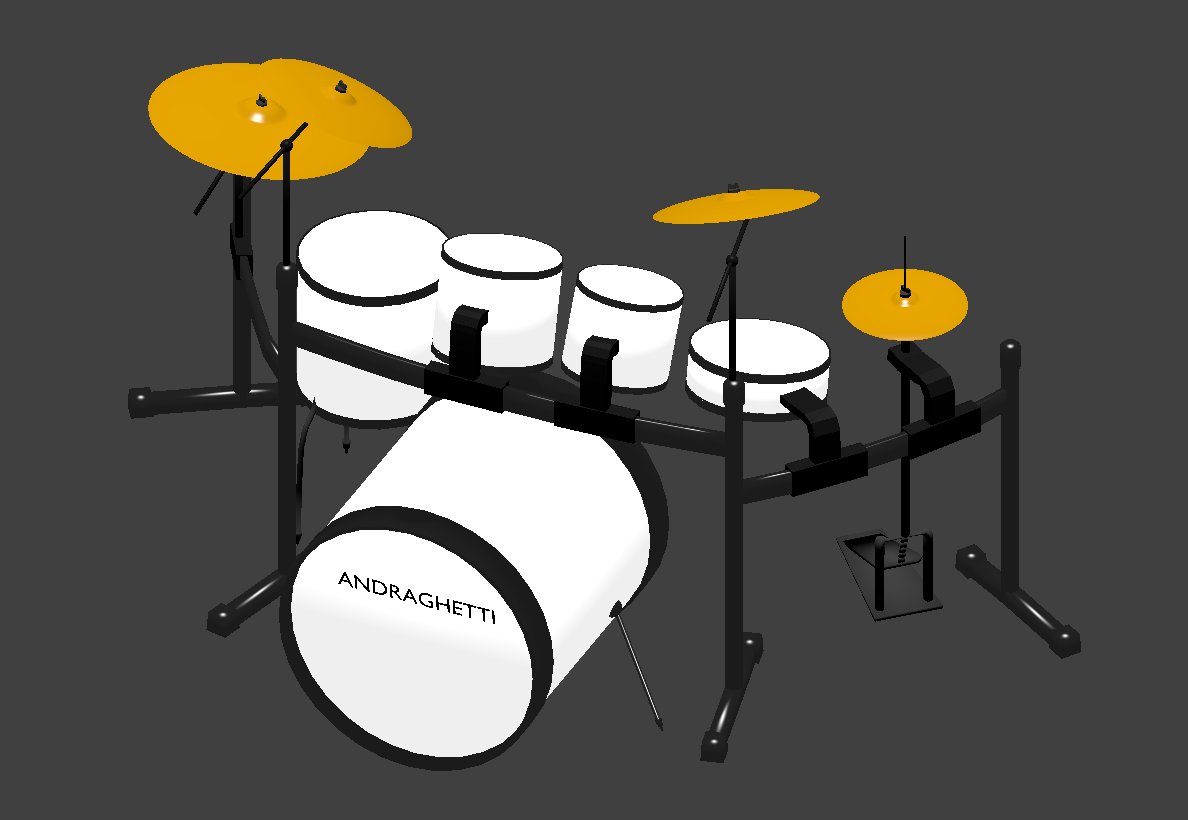
\includegraphics[height=6cm]{final1} }}%
    \subfloat[Retro]{{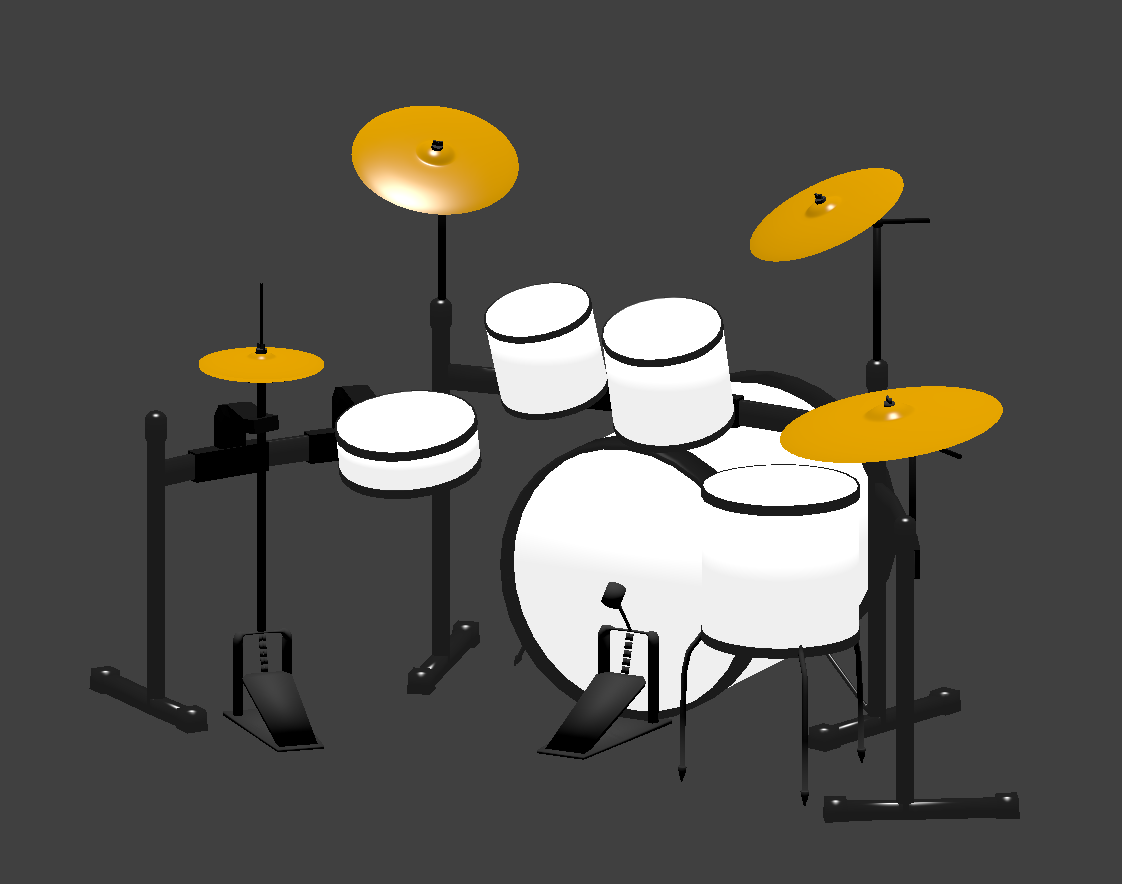
\includegraphics[height=6cm]{final2} }}%
	\vspace{-0.2cm}
\end{figure}

\subsection{Extrusion}
L'estrusione è stata utilizzata praticamente per tutte le parti della batteria esclusi i piatti. Selezionando una faccia o i vertici che la compongono è possibile estruderla nella direzione della sua normale, permettendo di costruire in modo incrementale delle mesh. Un esempio specifico si ha nella creazione delle aste che fermano la grancassa e nel rack:
\begin{figure}[hbt]
    \centering
    \subfloat[Durante l'estrusione]{{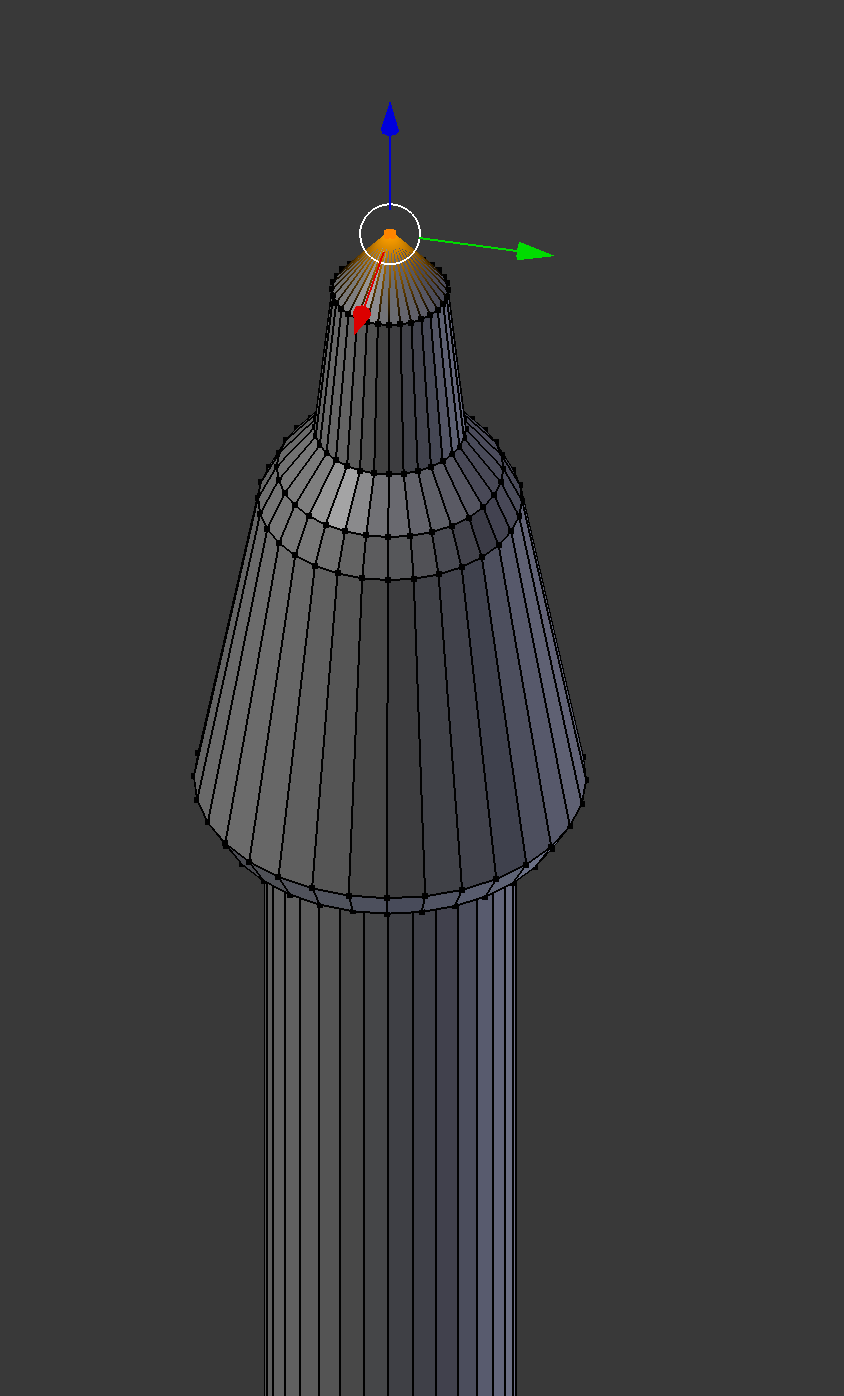
\includegraphics[height=6cm]{asta1} }}%
    \subfloat[Asta ultimata]{{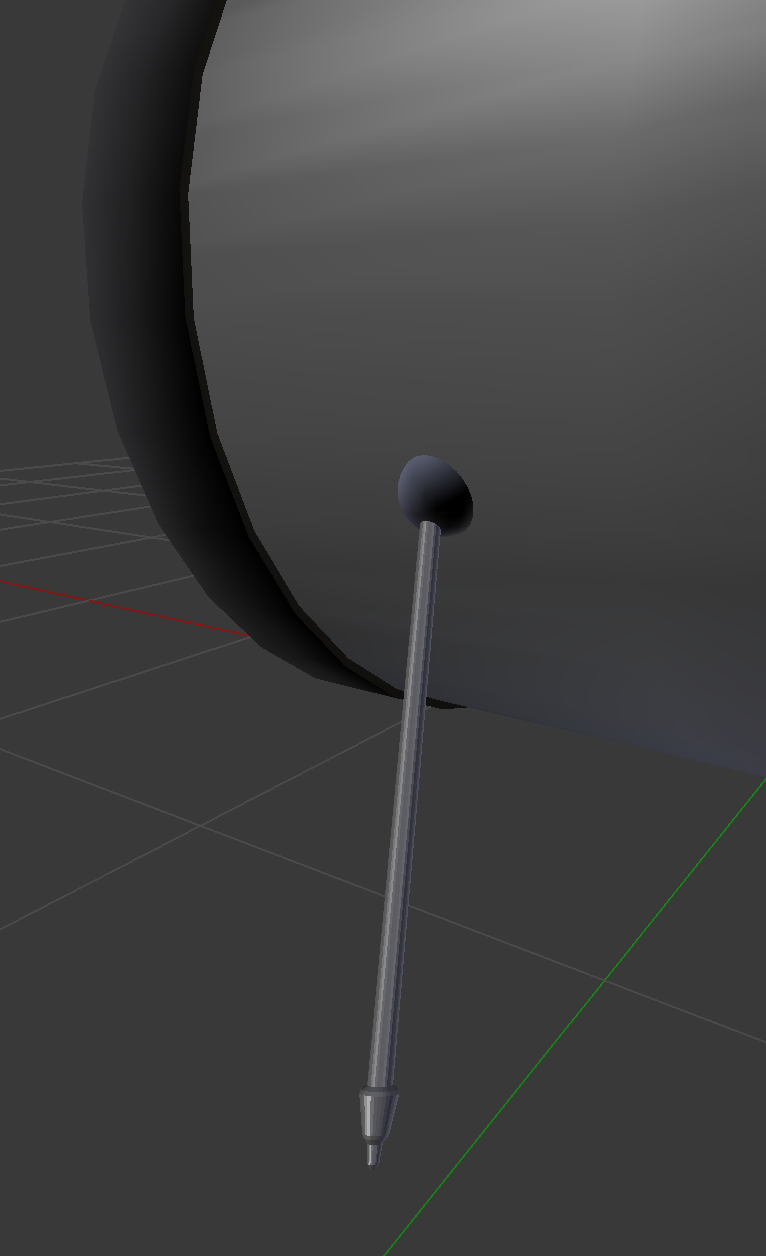
\includegraphics[height=6cm]{asta2} }}%
	\vspace{-0.2cm}
\end{figure}

\begin{figure}[hbt]
    \centering
    \subfloat[Durante l'estrusione]{{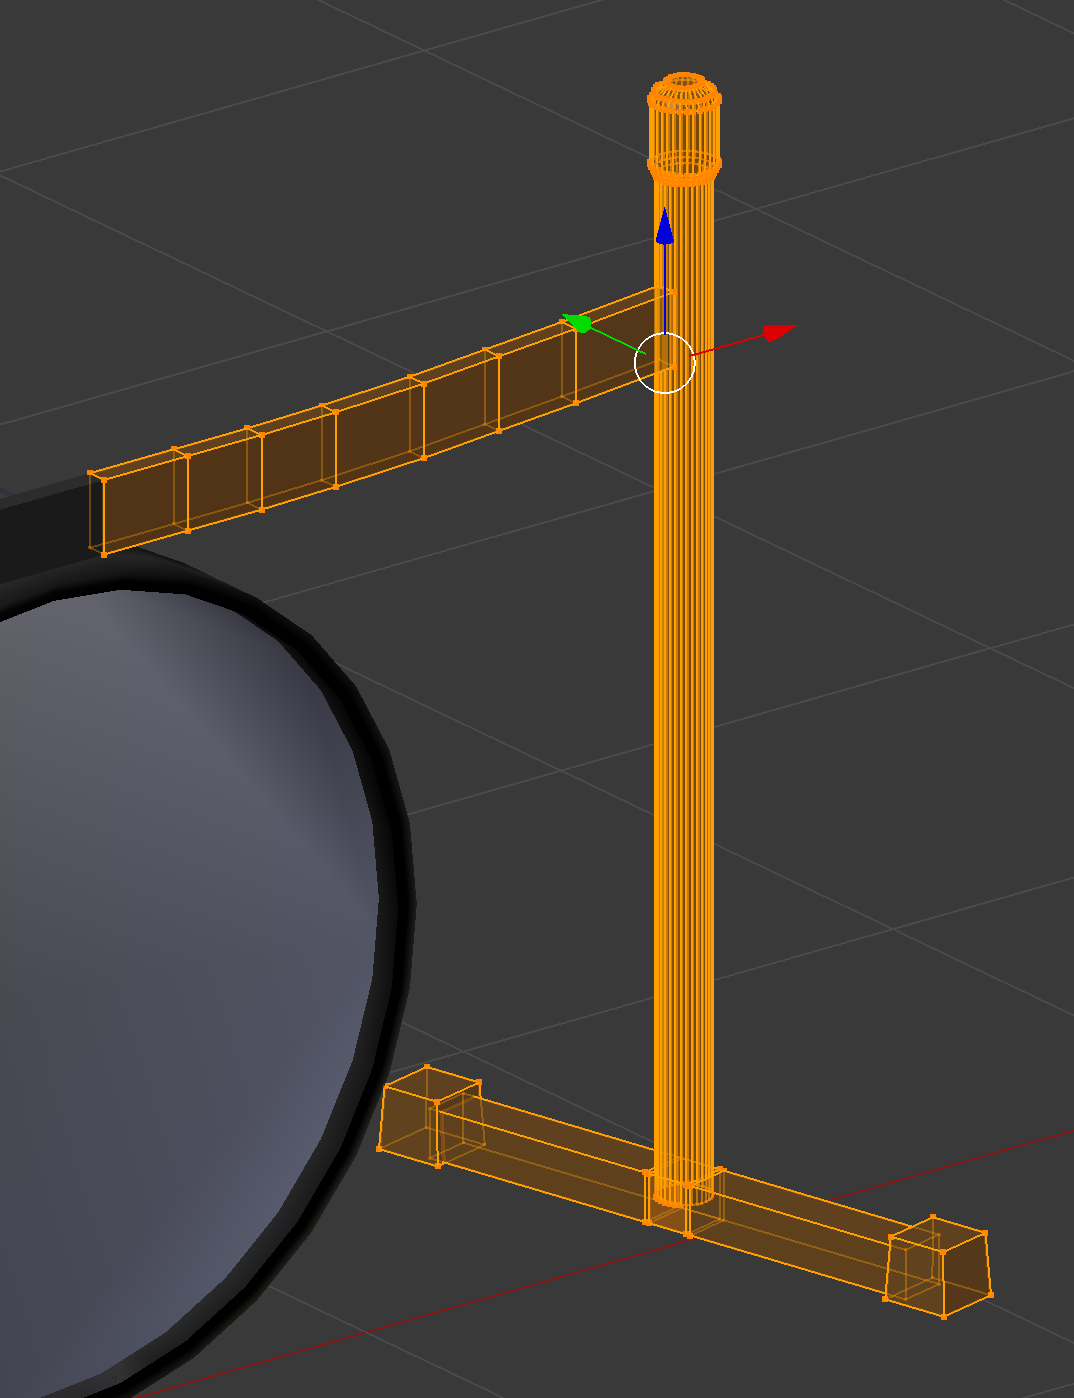
\includegraphics[height=6cm]{rack1} }}%
    \subfloat[Rack ultimato]{{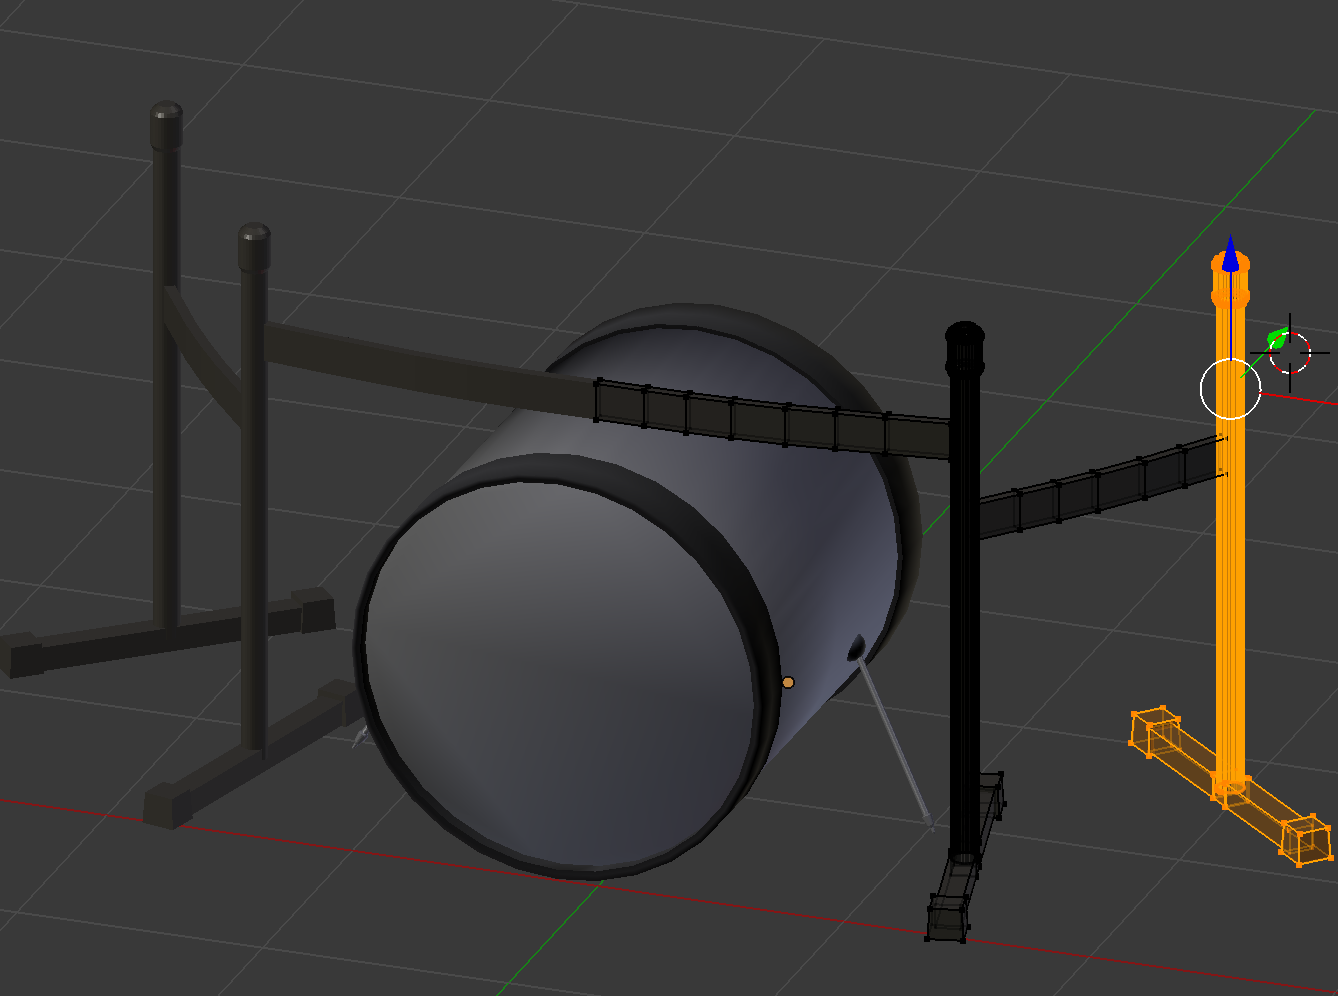
\includegraphics[height=6cm]{rack2} }}%
	\vspace{-0.2cm}
\end{figure}

Per molti elementi creati, si è utilizzata la funzione di mirroring per avere simmetria negli oggetti che lo richiedevano. Si può notare nell'immagine del Rack: Blender permette di creare e modificare una parte e la sua speculare viene creata automaticamente.


\newpage

\subsection{Spinning}
Per la parte di \textit{spinning} si è scelto di creare un piatto della batteria. Partendo da una curva NURBS è possibile modellare il profilo del piatto. Attivando la visualizzazione ortografica e trascinando sul piano di lavoro un'immagine del piatto, è possibile avere una base su cui modellare il piatto. (figura \ref{fig:nurbs})

 \begin{figure}[htb]
    \centering
    %\vspace{-0.7cm}
    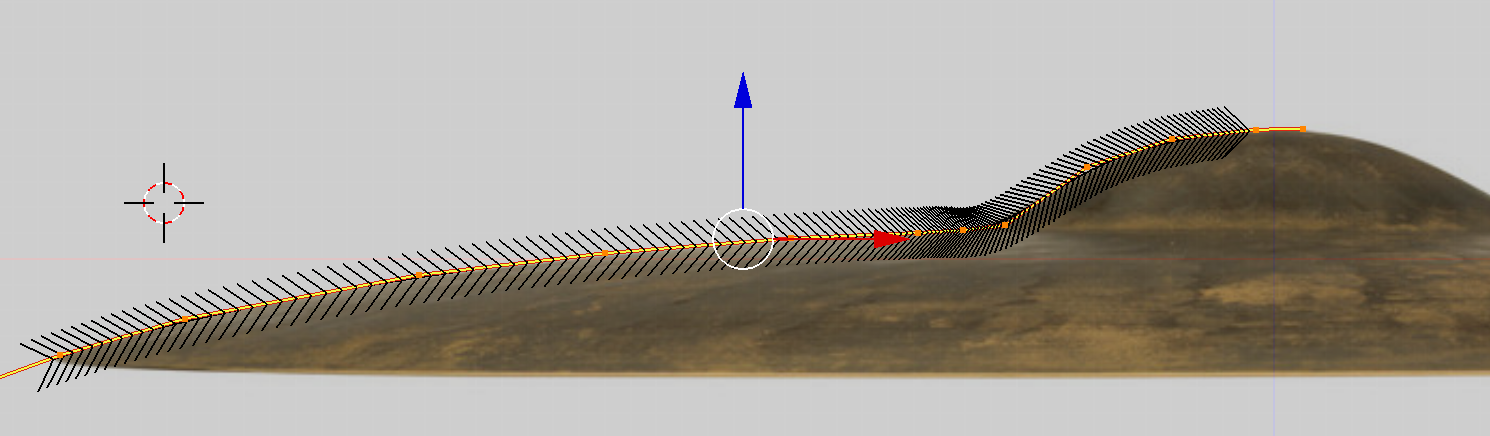
\includegraphics[width=\textwidth]{nurbs}
    \caption{\label{fig:nurbs}}
    %\vspace{-0.3cm}
\end{figure}

Una volta ottenuto il profilo perfetto, occorre convertire la curva in un oggetto mesh (alt + C) per poter effettuare lo \textit{spinning}. 

\begin{wrapfigure}{l}{0.3\textwidth} %this figure will be at the rightù
    \centering
    \vspace{-0.7cm}
    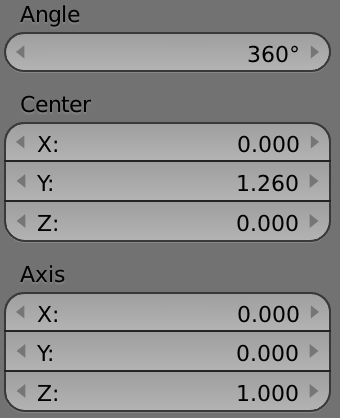
\includegraphics[height=5.5cm]{spin-values}
    \caption{\label{fig:spin-values}}
    \vspace{-3.7cm}
\end{wrapfigure}

\vspace{1cm}\noindent Come si può notare in figura \ref{fig:spin-values} è stata applicata una rotazione di 360\degree, è stato preso un centro di rotazione leggermente rialzato con un asse di rotazione unico $Z$.
La curva è stata traslata leggermente verso sinistra per poter lasciare un buco in alto. Questo buco serve per inserire il piatto su un asta che lo sorregge.\\

\vspace{3cm}Il risultato ottenuto è il seguente. Si può notare la differenza tra la vesione flat e la versione smooth. Nell'immagine con la versione flat si può notare ancora la NURBS trasformata in mesh.\\

\begin{figure}[hbt]%
	\vspace{-1cm}
    \centering
    \subfloat[Piatto Flat]{{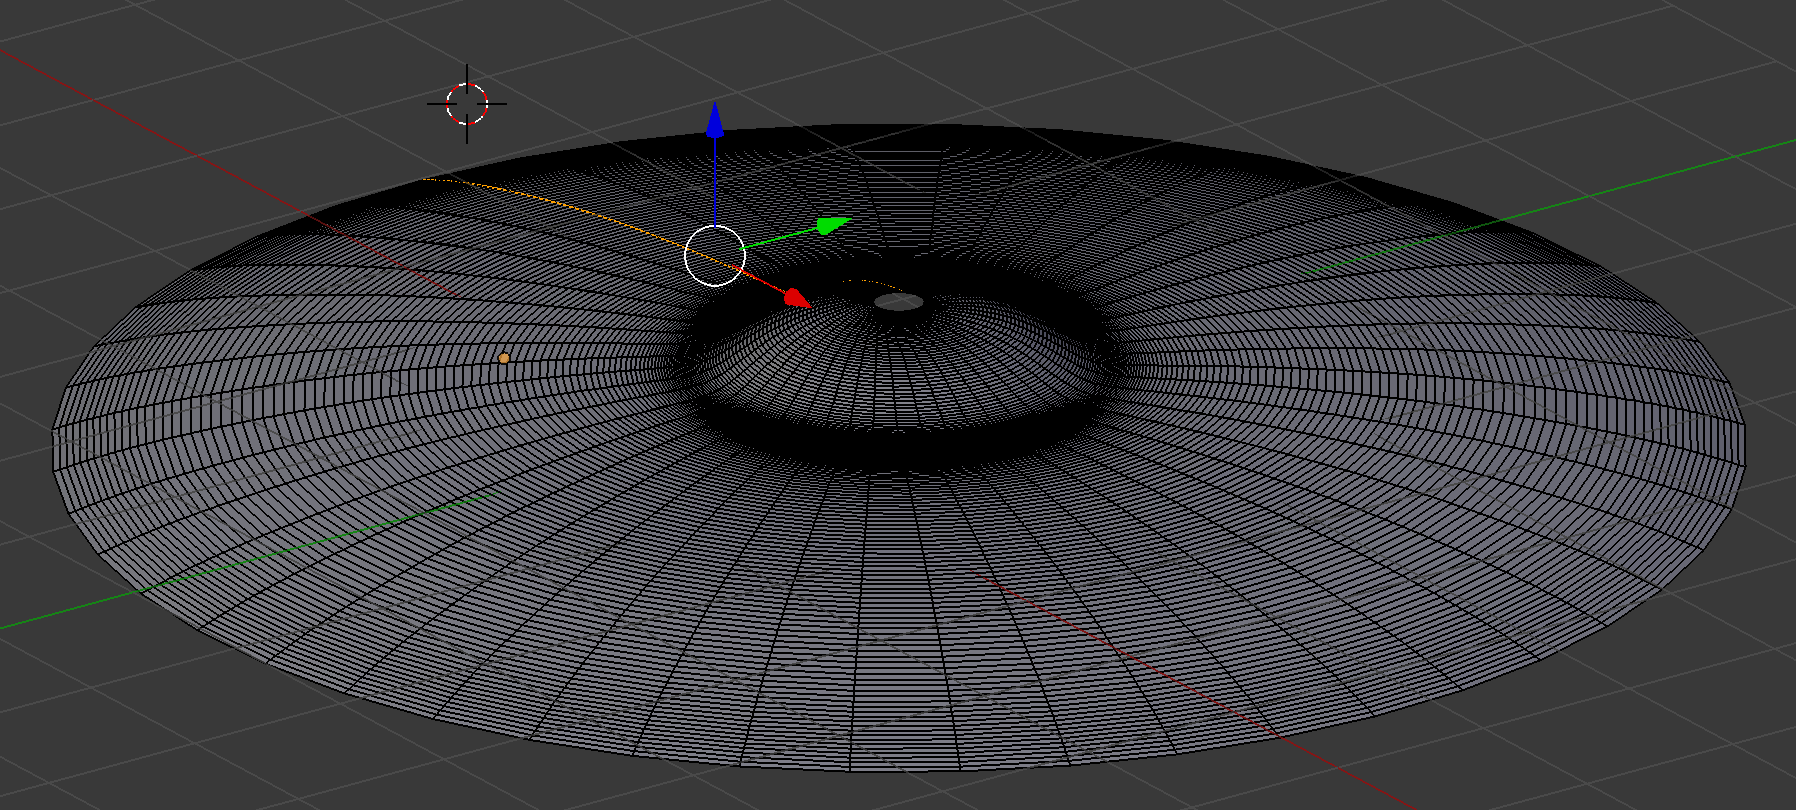
\includegraphics[height=3.5cm]{cymbal-flat} }}%
    \subfloat[Piatto Smooth]{{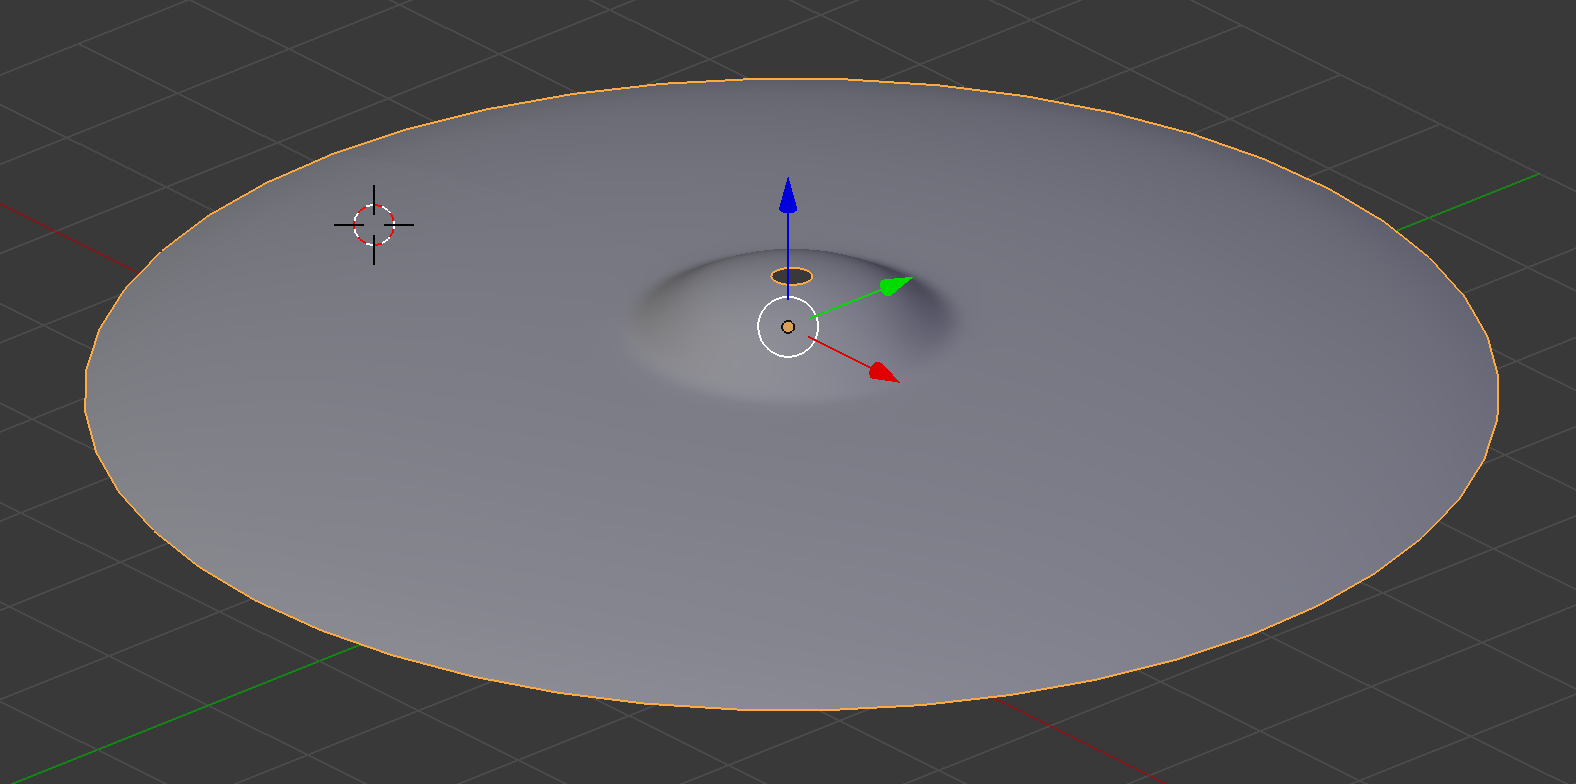
\includegraphics[height=3.5cm]{cymbal-smooth} }}%
	\vspace{-0.2cm}
\end{figure}


\newpage
%===========================
\section{Parte 2 - MeshLab}
L'esercitazione richiedeva di eseguire i seguenti punti con uno o più modelli:
\begin{itemize}
  \item Ricostruzione di oggetti mesh a partire da nuvole di punti (Poisson, MLS, Marching cubes)
  \item Utilizzare i tool Fill Hole/Mesh Repair per la chiusura di una mesh parzialmente corrotta
  \item FAIRING: Applicare un filtro di denoising (fairing) ad una mesh perturbata
  \item DECIMATION: Semplificare a più livelli una mesh con un numero elevato di elementi
  \item Utilizzare gli strumenti di misura della qualità della superficie (curvatura)
\end{itemize}

Come specificato, è stato scaricato un oggetto .xyz, ovvero una nuvola di punti dal sito \texttt{http://\-visionair\-.ge\-.imati.cnr.it/\-ontologies/\-shapes/releases.jsp} per il primo punto.

Importando l'oggetto scaricato dal sito si ha il risultato seguente:
 \begin{figure}[htb]
    \centering
    %\vspace{-0.7cm}
    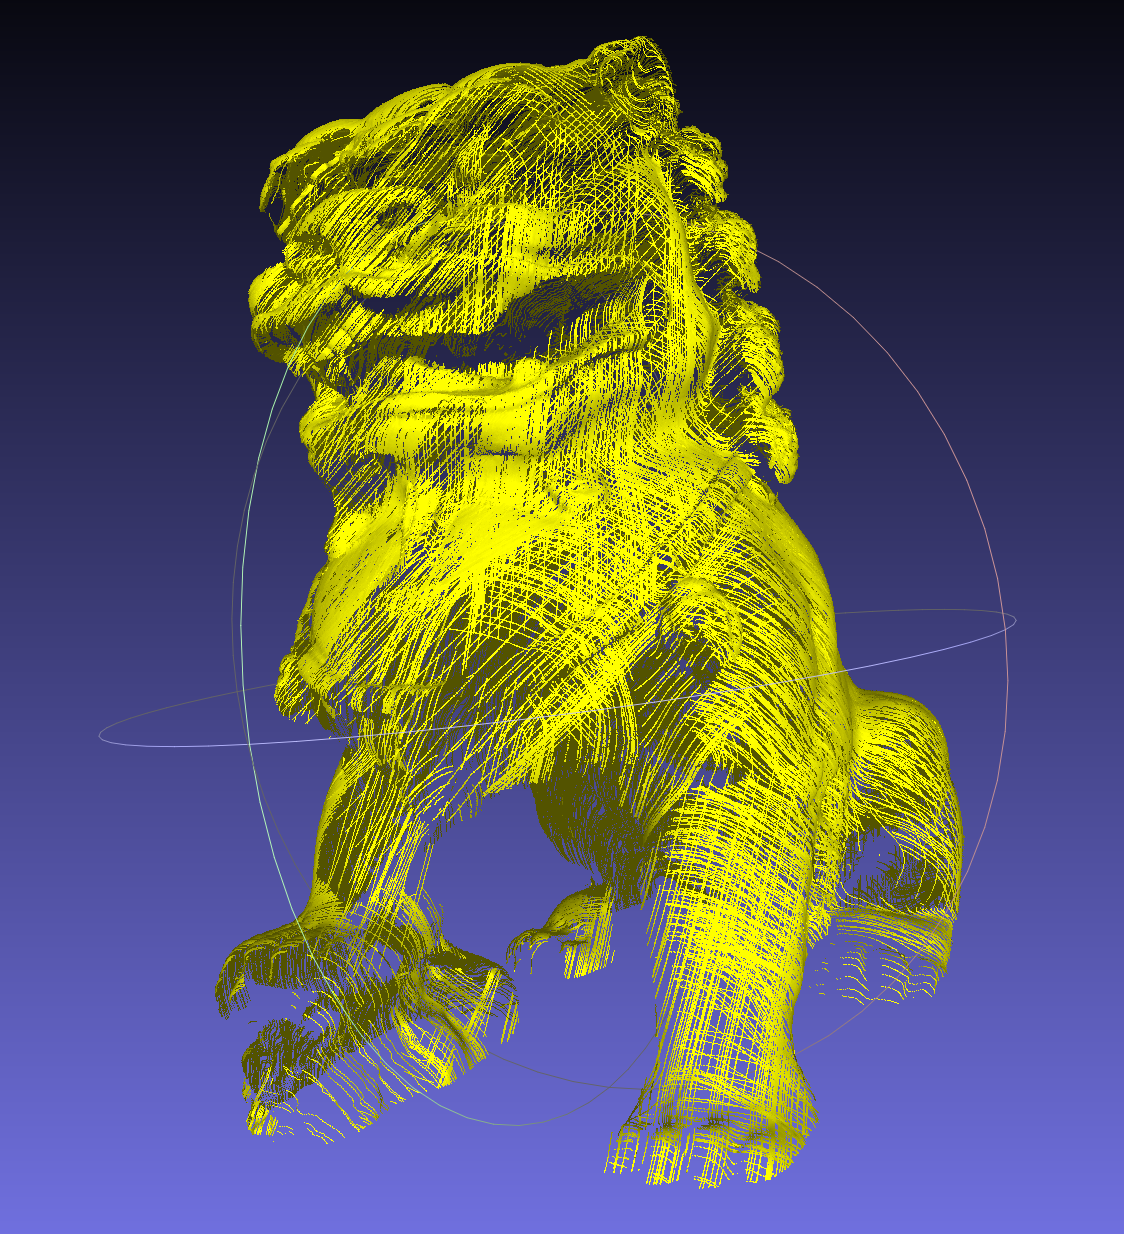
\includegraphics[width=0.6\textwidth]{begin}
    \caption{\label{fig:begin}}
    %\vspace{-0.3cm}
\end{figure}

\subsection{Ricostruzione Mesh}
Per ricostruire la mesh si è inizialmente applicato un campionamento per ridurre il numero di punti ed eseguire la ricostruzione in meno tempo. Inoltre è scritto sulla finestra dell'algoritmo utilizzato per ricostruire i triangoli della mesh che quest'ultimo lavora meglio su nuvole di punti campionate con Poisson: \texttt{Filters/Sampling/Poisson-disk Sampling} attivando \textit{Base Mesh Subsampling}.
\newpage

Campionando 30000 punti si ottiene:
 \begin{figure}[htb]
    \centering
    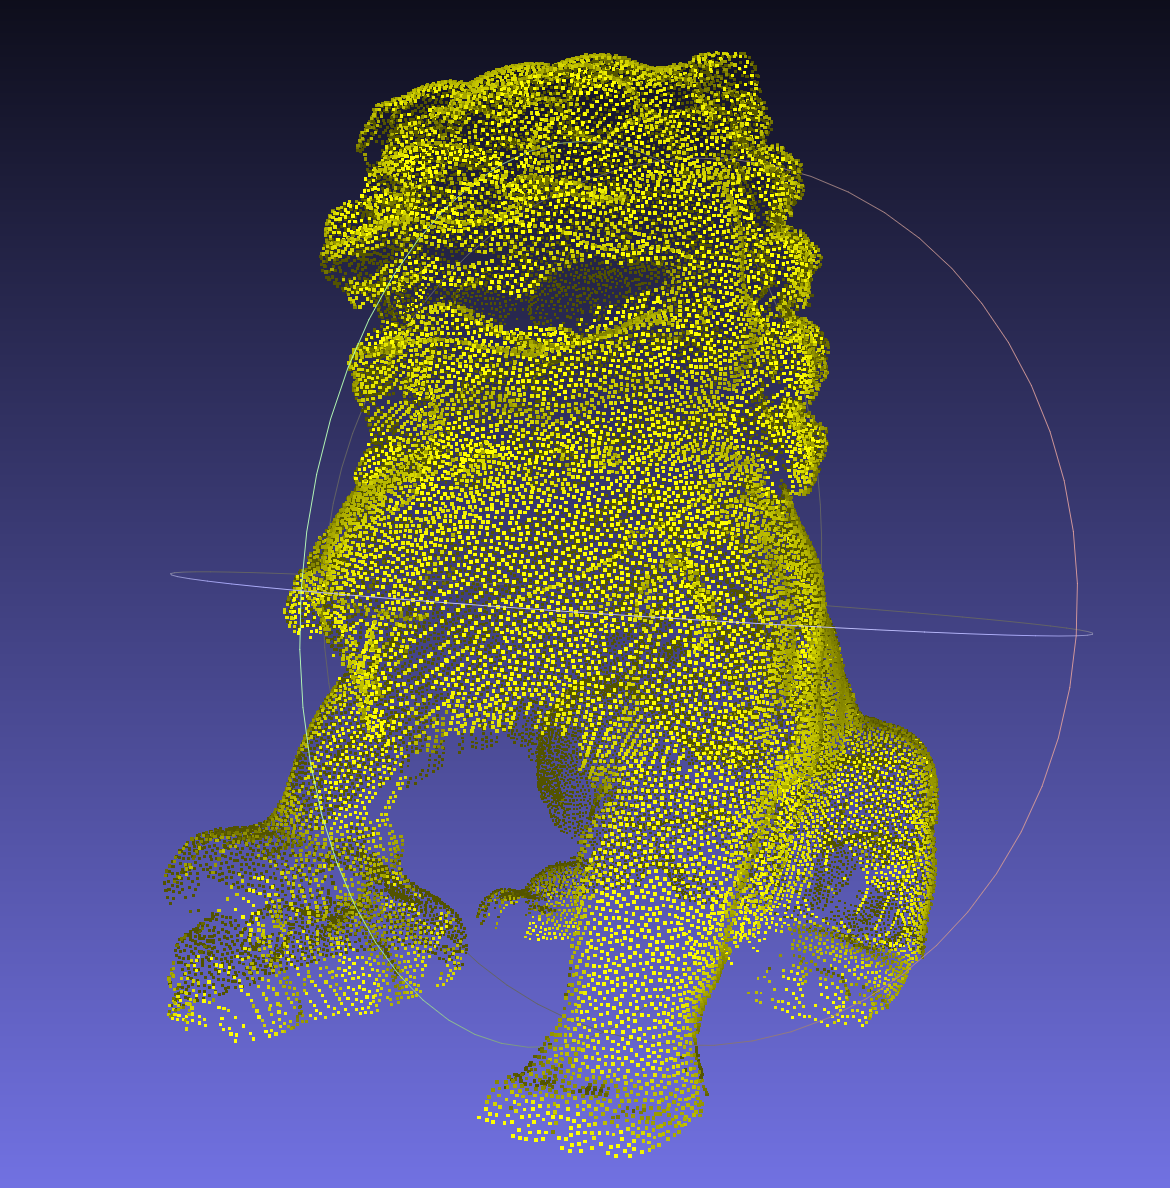
\includegraphics[width=0.5\textwidth]{poisson}
    \caption{\label{fig:poisson}}
    \vspace{-0.3cm}
\end{figure}

Per ricostruire la mesh è stato necessario ricalcolare le normali con il comando \texttt{Filters/\-Normals, \-Curvatures and \-Orientation/\-Calculate normals \-for \-point \-sets}. A questo punto occorre eseguire il comando \texttt{Filters/\-Remeshing, \-Semplification and \-Construction/\-Surface\- Recostruction\-: Ball \-Pivoting} per l'algoritmo di ricostruzione dei triangoli della mesh.

Il risultato è il seguente:
 \begin{figure}[htb]
    \centering
    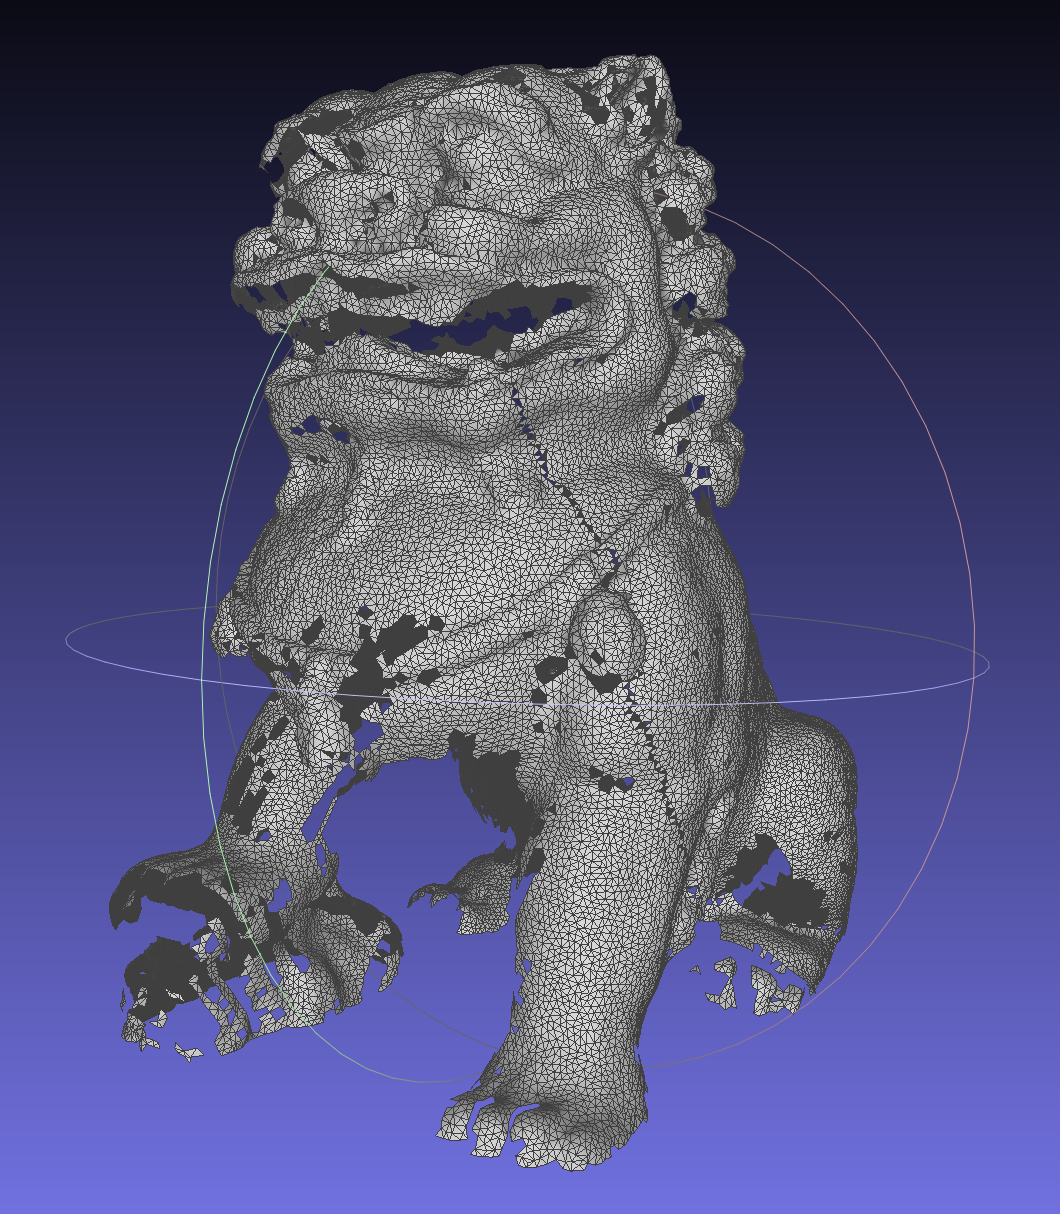
\includegraphics[width=0.5\textwidth]{mesh1}
    \caption{\label{fig:mesh}}
    \vspace{-0.3cm}
\end{figure}

\subsection{Fill Hole}
Alternando il ricalcolo delle normali e il comando per riparare i buchi (\texttt{Filters/\-Remeshing, \-Semplification\- and \-Construction/Close Holes}), si è ottenuto il seguente risultato parziale:
\begin{figure}[hbt]
    \centering
    \subfloat[Prima]{{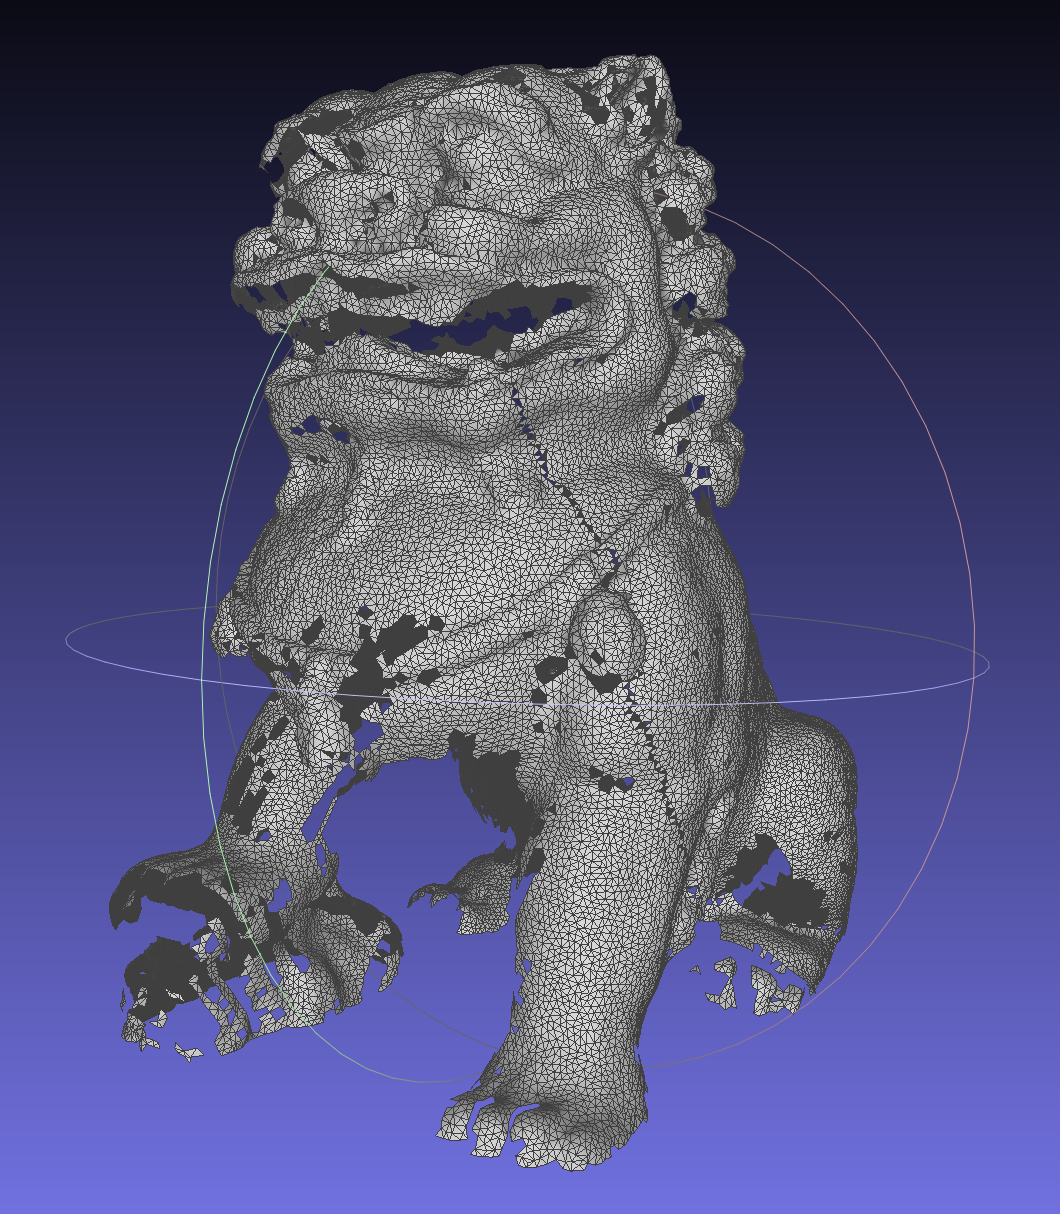
\includegraphics[height=7cm]{mesh1} }}%
    \subfloat[Dopo]{{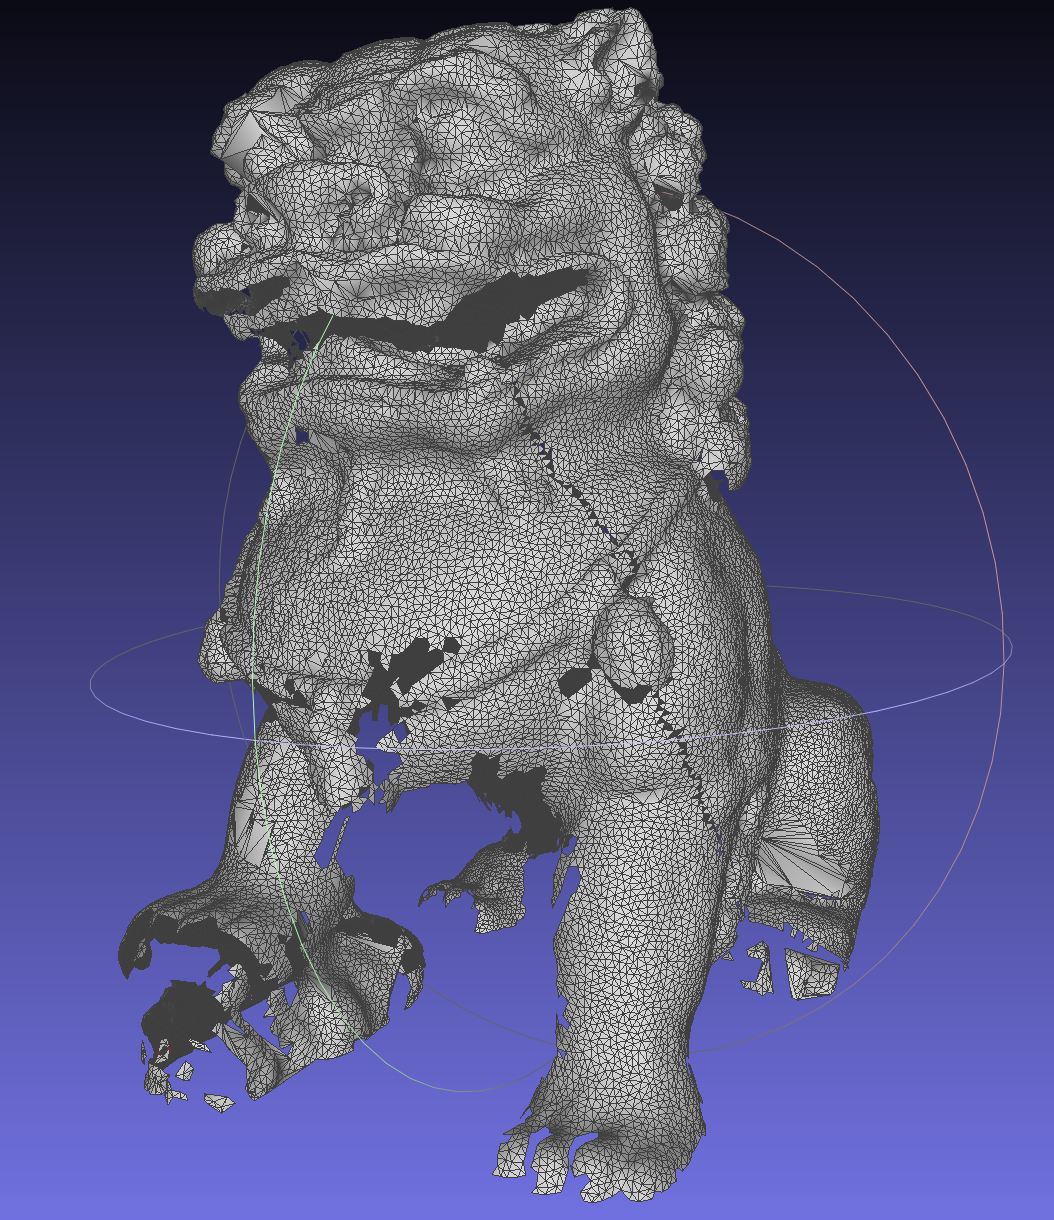
\includegraphics[height=7cm]{holes} }}%
	\vspace{-0.2cm}
\end{figure}


\subsection{Fairing}
Per questo punto dell'esercitazione si è utilizzata la mesh \texttt{stell2perturb.obj} presente nel template.
Si è scelto di applicare il denoising Laplaciano con il comando \texttt{Filters/\-Smoothing, \-Fairing \-and \-Deformation/\-Laplacian \-Smooth}

\begin{figure}[hbt]
    \centering
    \subfloat[Prima]{{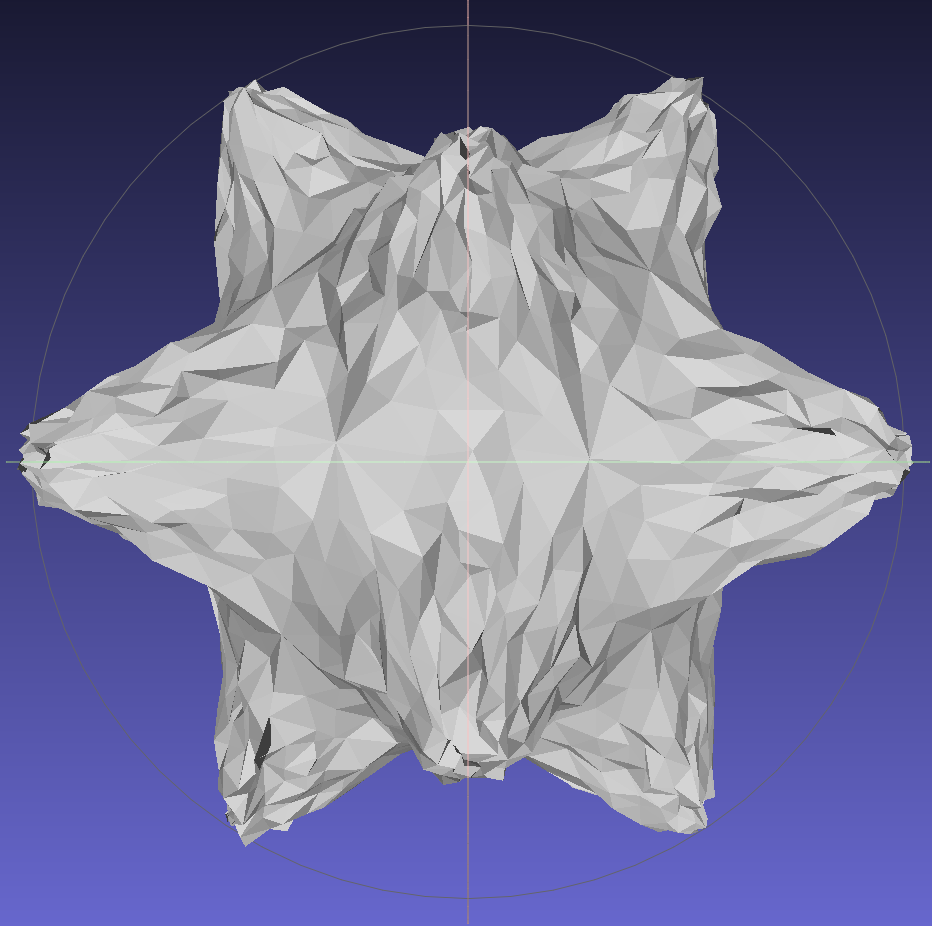
\includegraphics[height=5cm]{star1} }}%
    \subfloat[Dopo 1]{{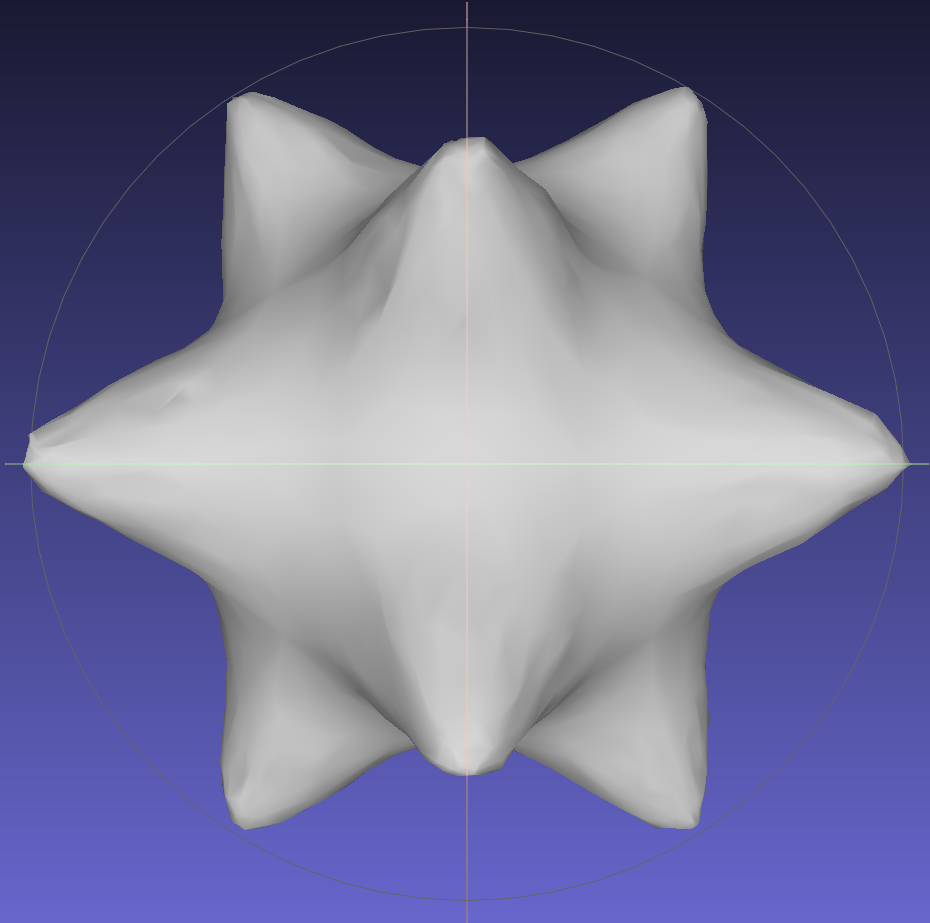
\includegraphics[height=5cm]{star2} }}%
    \subfloat[Dopo 3]{{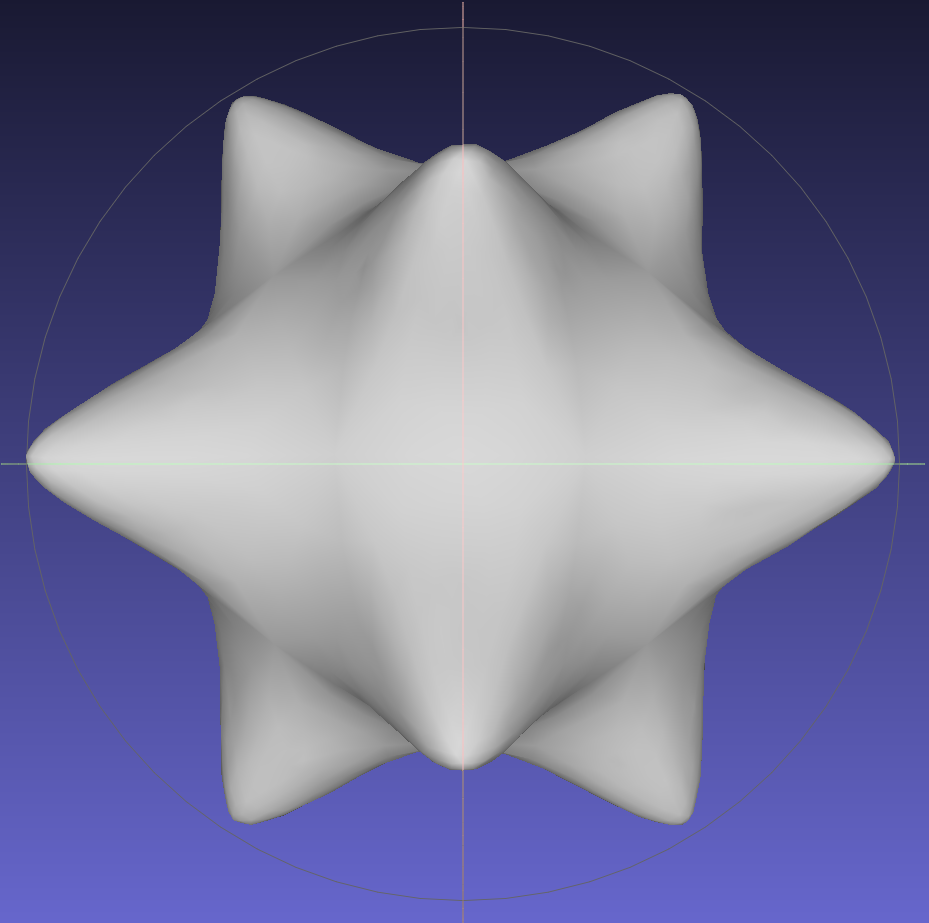
\includegraphics[height=5cm]{star3} }}%
	\vspace{-0.2cm}
\end{figure}

\newpage
\subsection{Decimation}
Per questo punto dell'esercitazione si è utilizzata la mesh \texttt{igea.obj} presente nel template. Si è scelto di applicare il filtro che riduce il numero di facce tramite la \textit{Quadric Edge Collapse Decimation} con il comando: \texttt{Filters/\-Remeshing, \-Semplification\- and \-Construction/\-Quadric \-Edge \-Collapse \-Decimation}.

\begin{figure}[hbt]
    \centering
    \subfloat[33585 facce]{{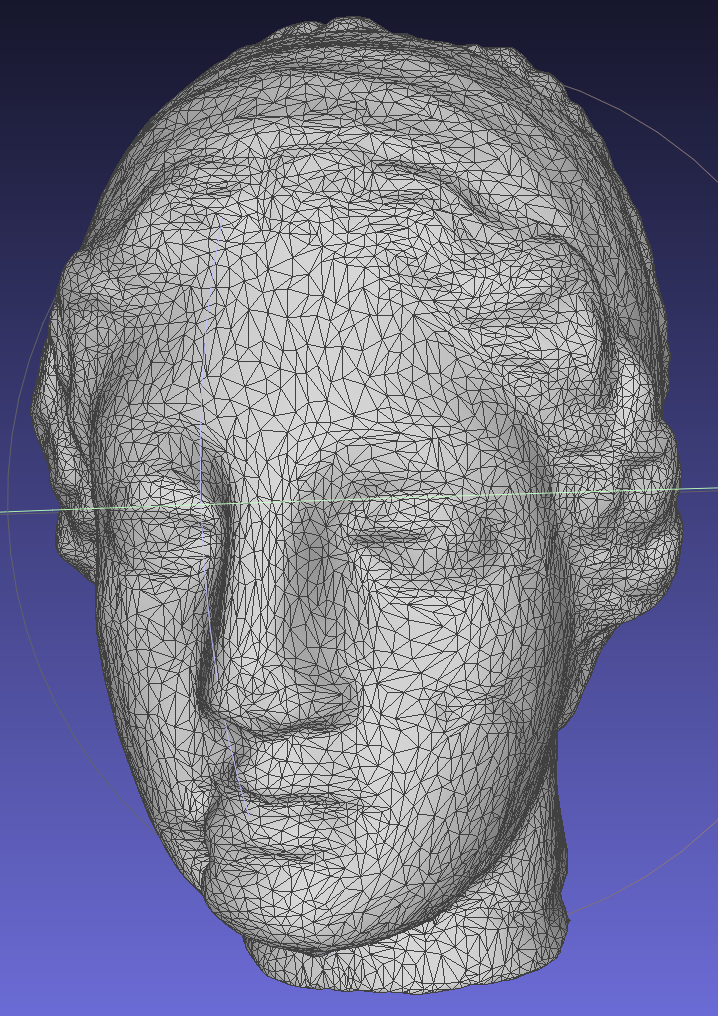
\includegraphics[height=8cm]{igea1} }}%
    \subfloat[16792 facce]{{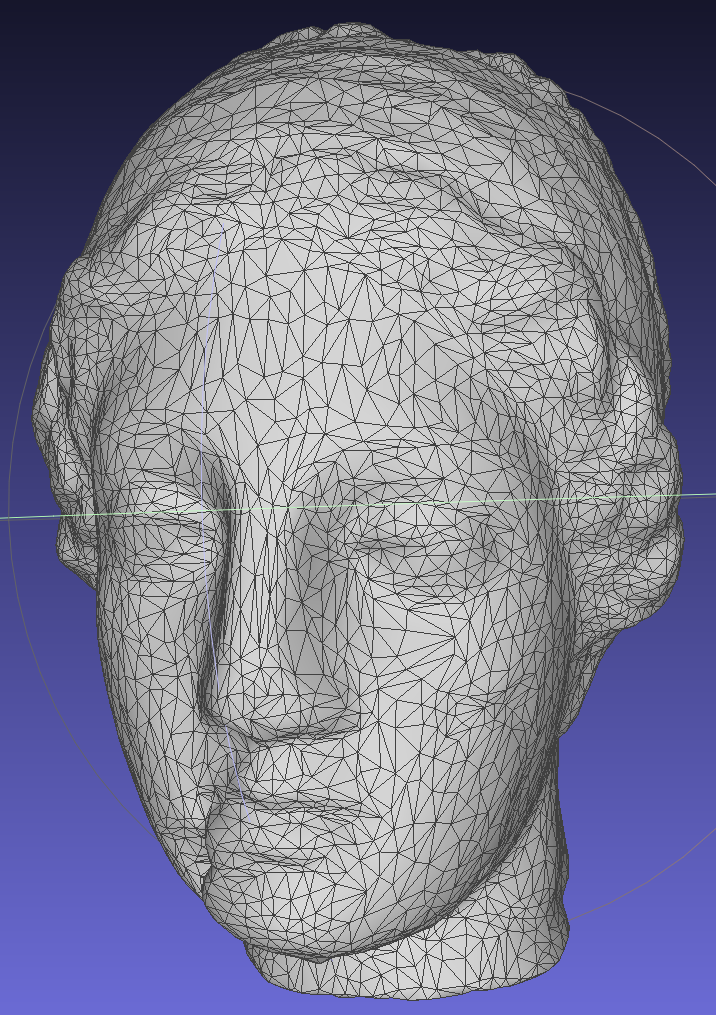
\includegraphics[height=8cm]{igea2} }}%
    \subfloat[4198 facce]{{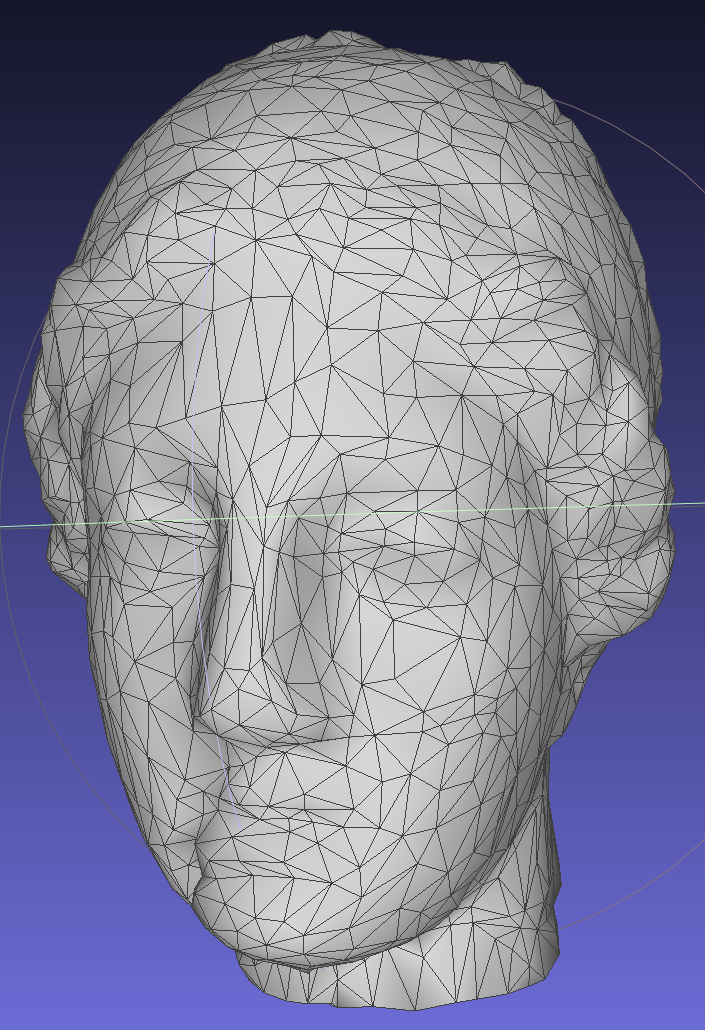
\includegraphics[height=8cm]{igea3} }}%
	\vspace{-0.2cm}
\end{figure}

\subsection{Strumenti di curvatura}
Per questo punto dell'esercitazione si è utilizzata la mesh \texttt{mannequin.obj} presente nel template. Meshlab mette a disposizione 4 tipi di curvatura utilizzando il comando \texttt{Filters/\-Normals, \-Curvatures and \-Orientation/\-Discrete \-Curvature}:

\begin{figure}[hbt]
    \centering
    \subfloat[Mean Curvature]{{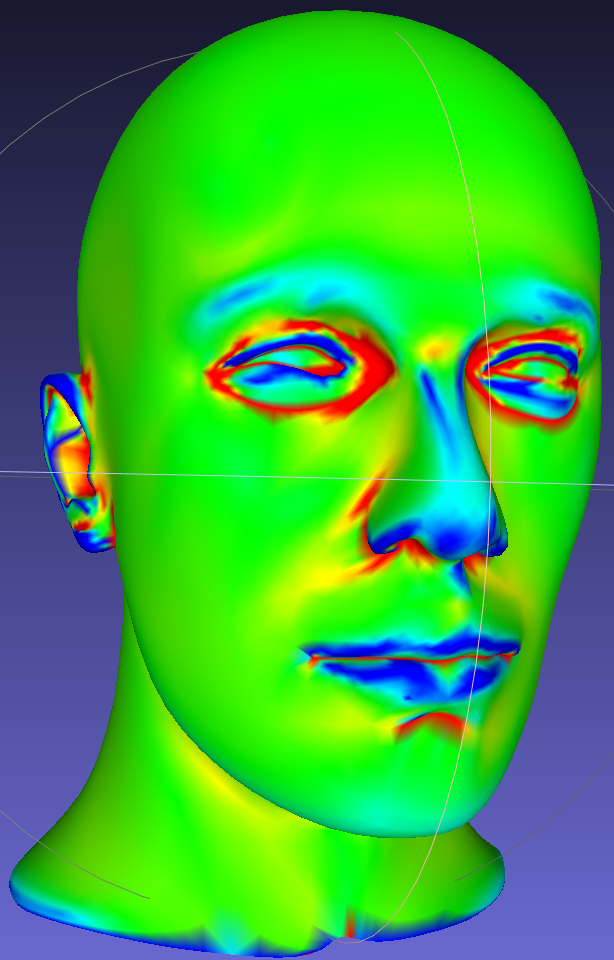
\includegraphics[height=6cm]{curv1} }}%
    \subfloat[Gaussian Curvature]{{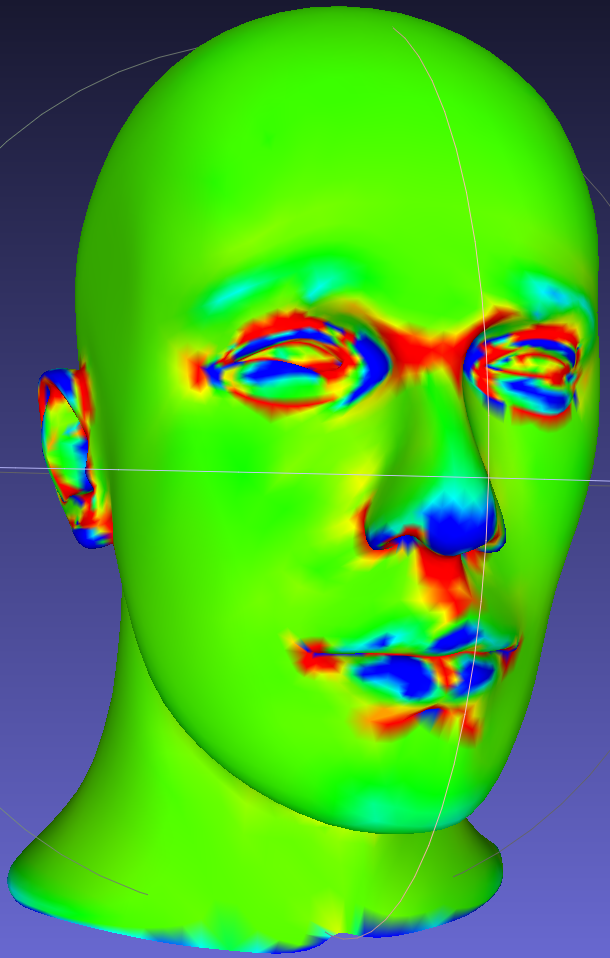
\includegraphics[height=6cm]{curv2} }}%
    \subfloat[RMS Curvature]{{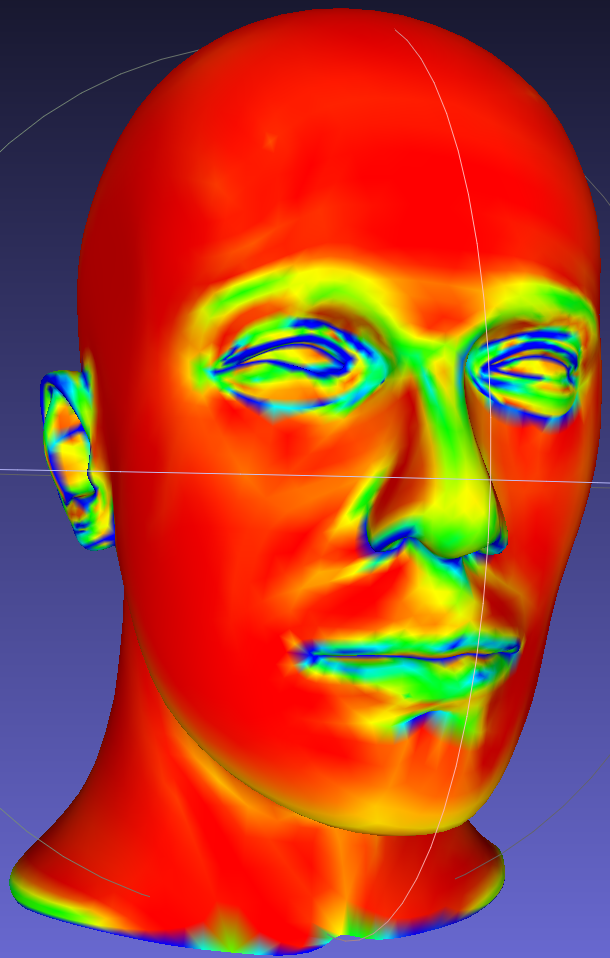
\includegraphics[height=6cm]{curv3} }}%
    \subfloat[ABS Curvature]{{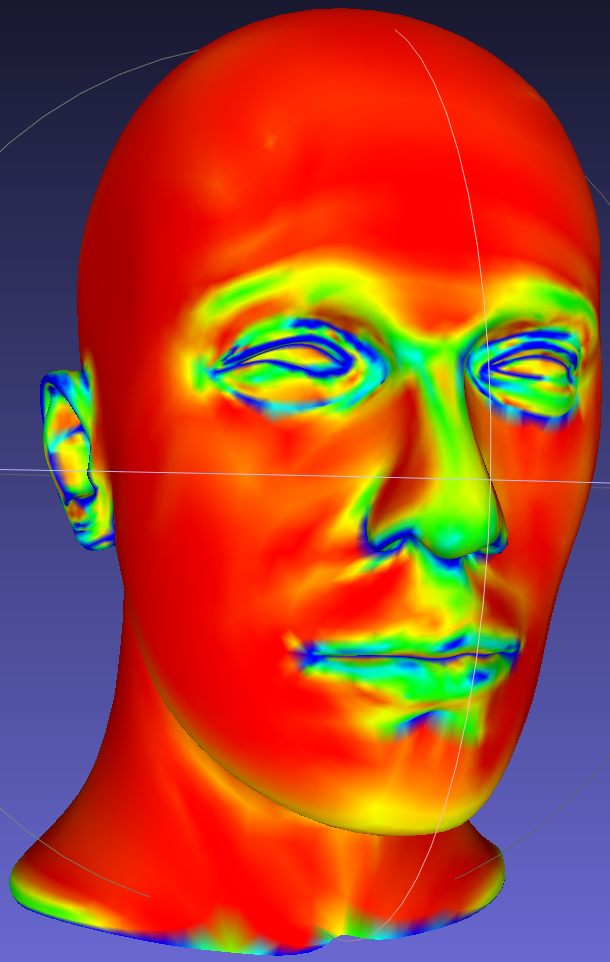
\includegraphics[height=6cm]{curv4} }}%
	\vspace{-0.2cm}
\end{figure}












%


